% 05 Implementation
\section{5. Solution Development}

\begin{enumerate}
    \item \textbf{Phase 1}: Data collection infrastructure (GPS Monitor)
    \item \textbf{Phase 2}: MAVLink UDP Bridge (overcame PX4 upstream changes)
    \item \textbf{Phase 3}: Inspector Tool for Docker management
    \item \textbf{Phase 4}: Auto-labeling system development
    \item \textbf{Phase 5}: Machine learning pipeline (RF + CNN)
    \item \textbf{Phase 6}: Live inference engine
    \item \textbf{Phase 7}: Dashboard development (Streamlit)
    \item \textbf{Phase 8}: System integration (TUI)
    \item \textbf{Phase 9}: Testing and validation
    \item \textbf{Phase 10}: Breaking point analysis (key research contribution)
\end{enumerate}

\begin{table}[H]
    \centering
    \caption{Research Timeline (5 meetings)}
    \label{tab:timeline}
    \begin{tabular}{|p{2cm}|p{3cm}|p{8cm}|}
        \hline
        \textbf{Week} & \textbf{Date} & \textbf{Key Achievements} \\
        \hline
        1 & 13 Mar 2026 & Confirmed ML approach, reviewed LSTM papers, planned Docker setup \\
        \hline
        2 & 19 Mar 2026 & Inspector Tool built, MAVLink UDP Bridge proposed (critical fix) \\
        \hline
        3 & 26 Mar 2026 & Telemetry pipeline operational, dataset creation started, ML baseline infrastructure \\
        \hline
        4 & 3 Apr 2026 & RF + CNN models trained (100\% accuracy), live inference pipeline, Streamlit UI \\
        \hline
        5 & 10 Apr 2026 & Full system demonstrated, breaking point contribution confirmed, presentation prepared \\
        \hline
    \end{tabular}
\end{table}

\begin{figure}[htbp]
    \centering
    \simplebox{
    \centering
    \textbf{Research Project Timeline}\\[0.5em]
    \begin{tabular}{|c|c|p{6cm}|}
        \hline
        \textbf{Week} & \textbf{Date} & \textbf{Key Achievements} \\
        \hline
        1 & 13 Mar 2026 & Confirmed ML approach, reviewed papers, planned Docker setup \\
        \hline
        2 & 19 Mar 2026 & Inspector Tool, MAVLink Bridge proposed (critical fix) \\
        \hline
        3 & 26 Mar 2026 & Telemetry pipeline operational, dataset creation started \\
        \hline
        4 & 3 Apr 2026 & RF+CNN models trained (100\% accuracy), live inference pipeline \\
        \hline
        5 & 10 Apr 2026 & Full system demonstrated, breaking point confirmed \\
        \hline
    \end{tabular}
    }
    \caption{Research Timeline (5 meetings)}
    \label{fig:timeline}
\end{figure}

\subsection{5.2 Technology Stack}

\begin{table}[htbp]
    \centering
    \caption{Technology Stack}
    \label{tab:tech_stack}
    \begin{tabular}{|l|l|p{5cm}|}
        \hline
        \textbf{Component} & \textbf{Technology} & \textbf{Purpose} \\
        \hline
        Simulation & PX4 SITL, Gazebo, Docker & Flight stack simulator \\
        \hline
        Telemetry Collection & Python, pymavlink & MAVLink protocol handling \\
        \hline
        Container Management & Custom Inspector Tool & Docker UI management \\
        \hline
        Data Processing & pandas, numpy & CSV processing, feature extraction \\
        \hline
        ML Training & scikit-learn, PyTorch & RF and CNN model training \\
        \hline
        Model Serialization & joblib & Model persistence \\
        \hline
        Dashboard & Streamlit & Web UI development \\
        \hline
        TUI Interface & Rich library & Terminal management interface \\
        \hline
        Configuration & YAML & System configuration management \\
        \hline
\end{tabular}
\end{table}

\begin{figure}[htbp]
    \centering
    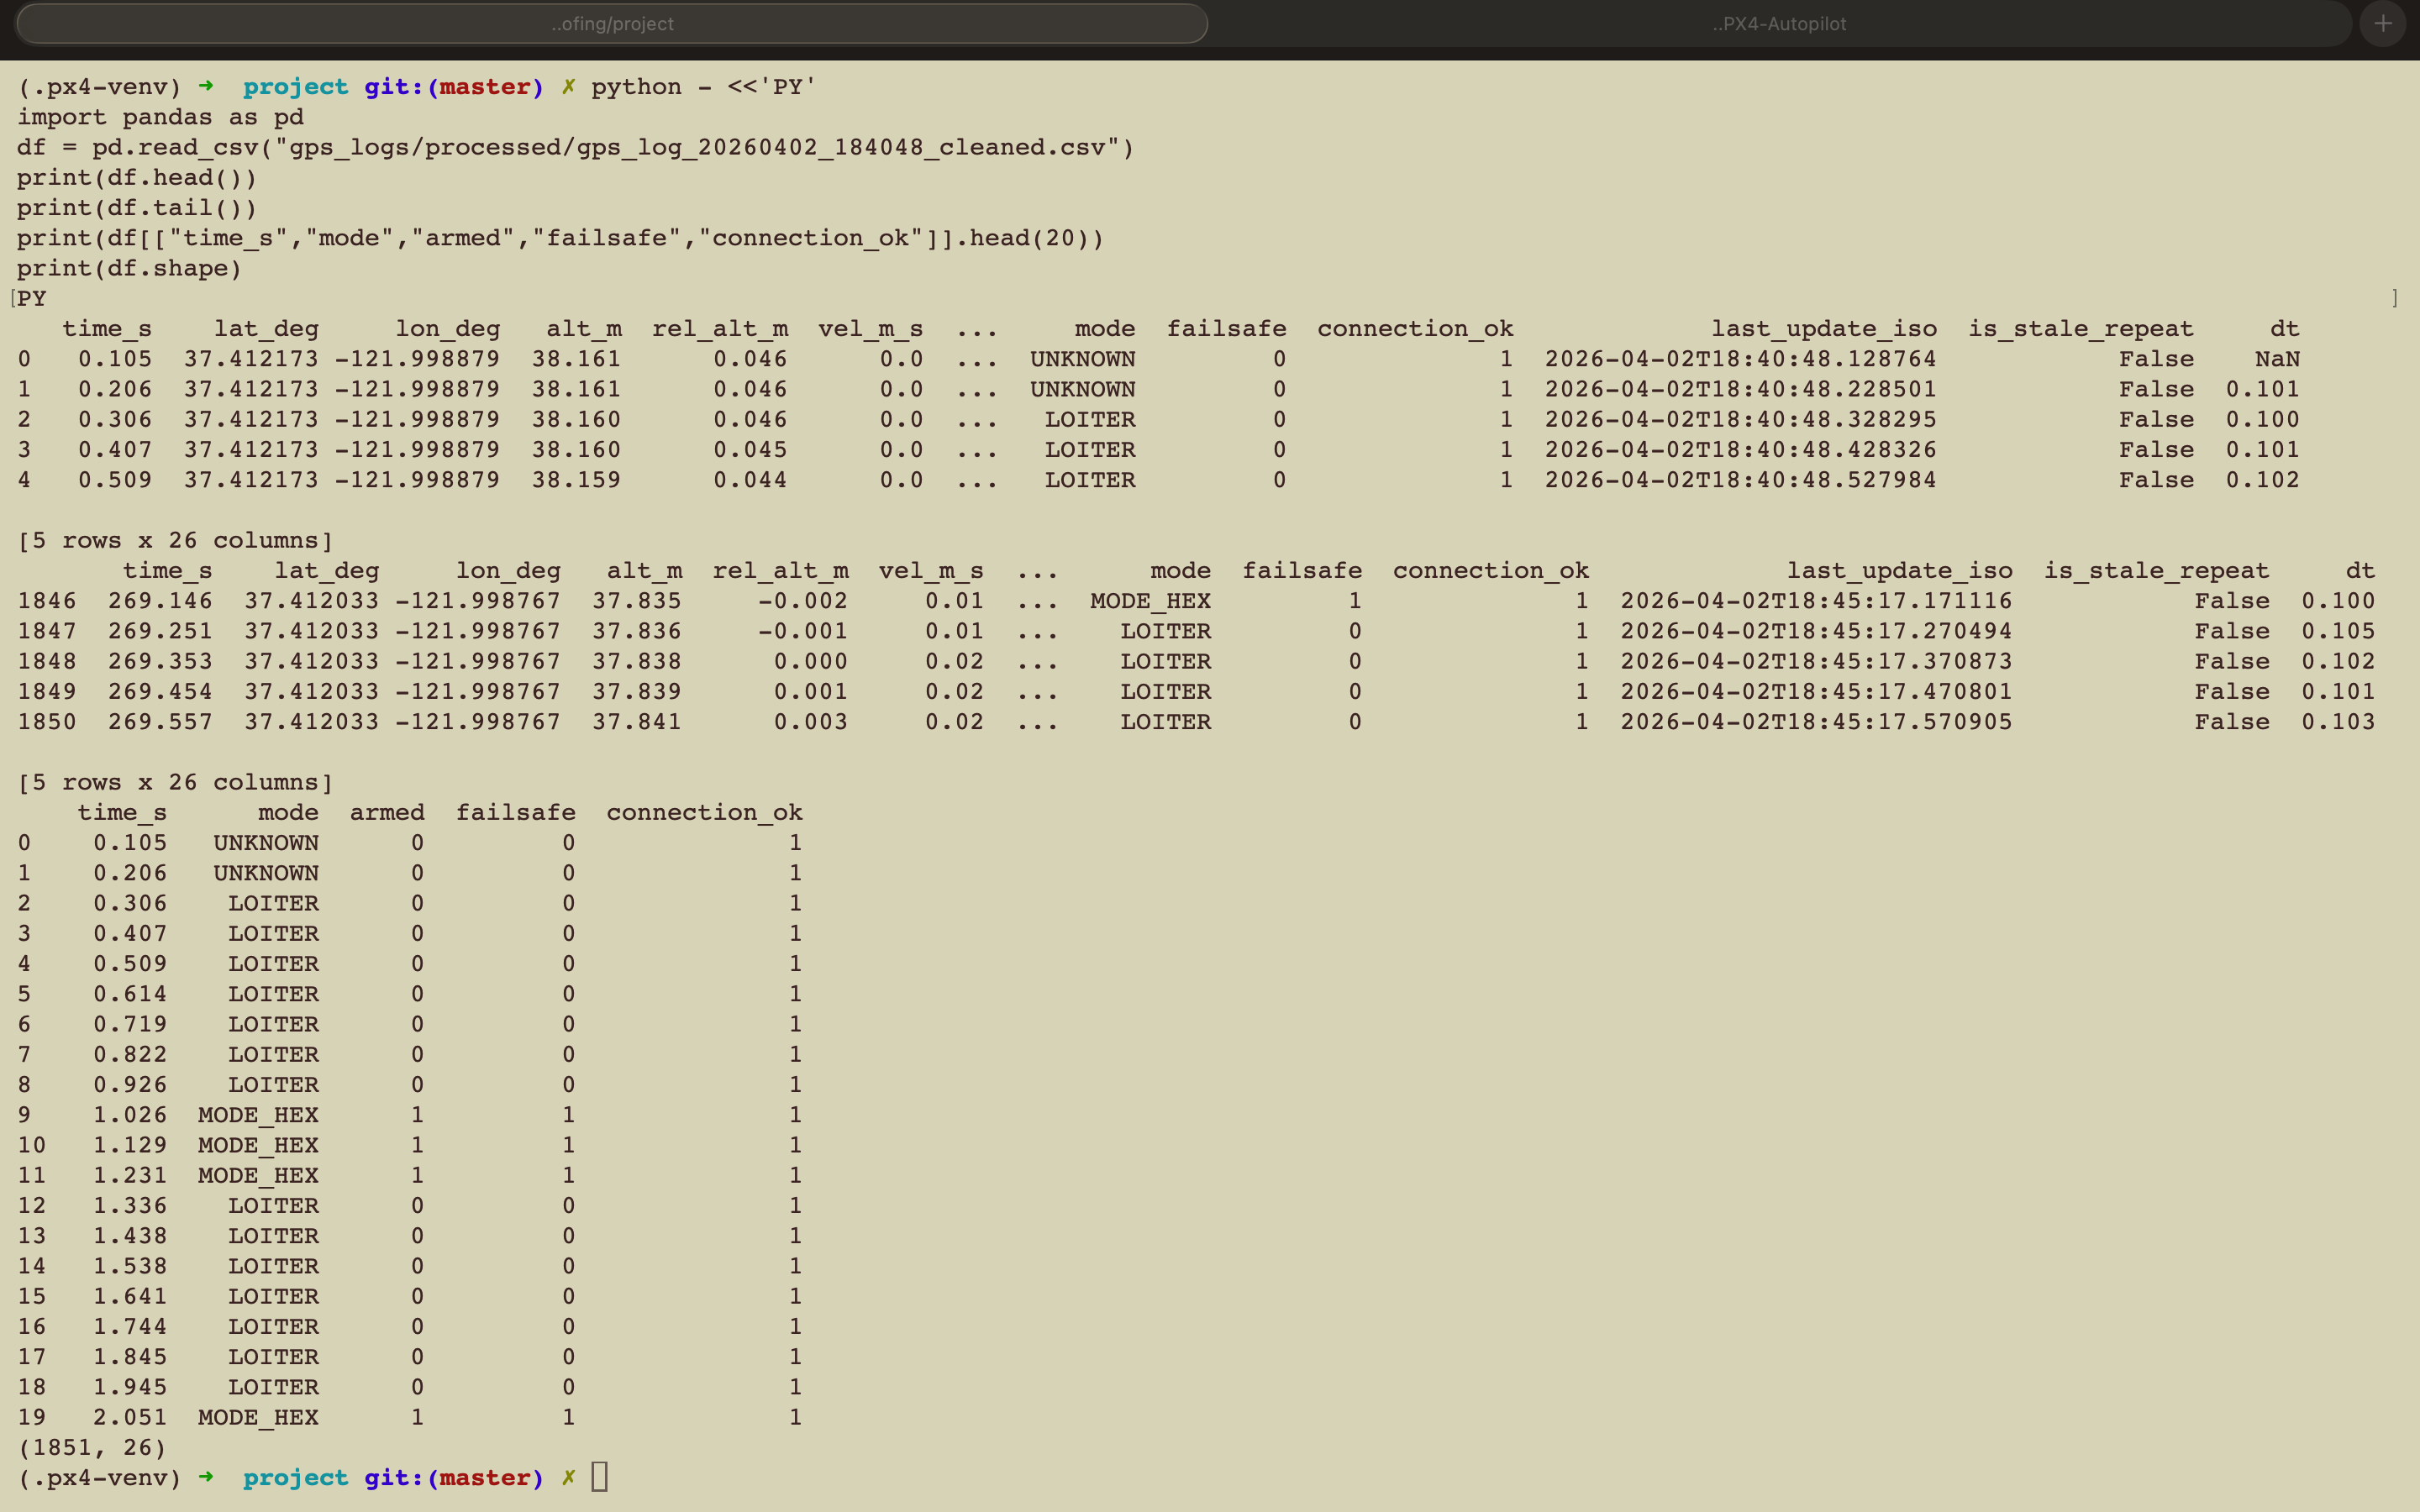
\includegraphics[width=0.7\linewidth]{figures/inspect the cleaned csv.png}
    \caption{Inspection of cleaned CSV telemetry dataset}
    \label{fig:cleaned_csv}
\end{figure}

\begin{figure}[htbp]
    \centering
    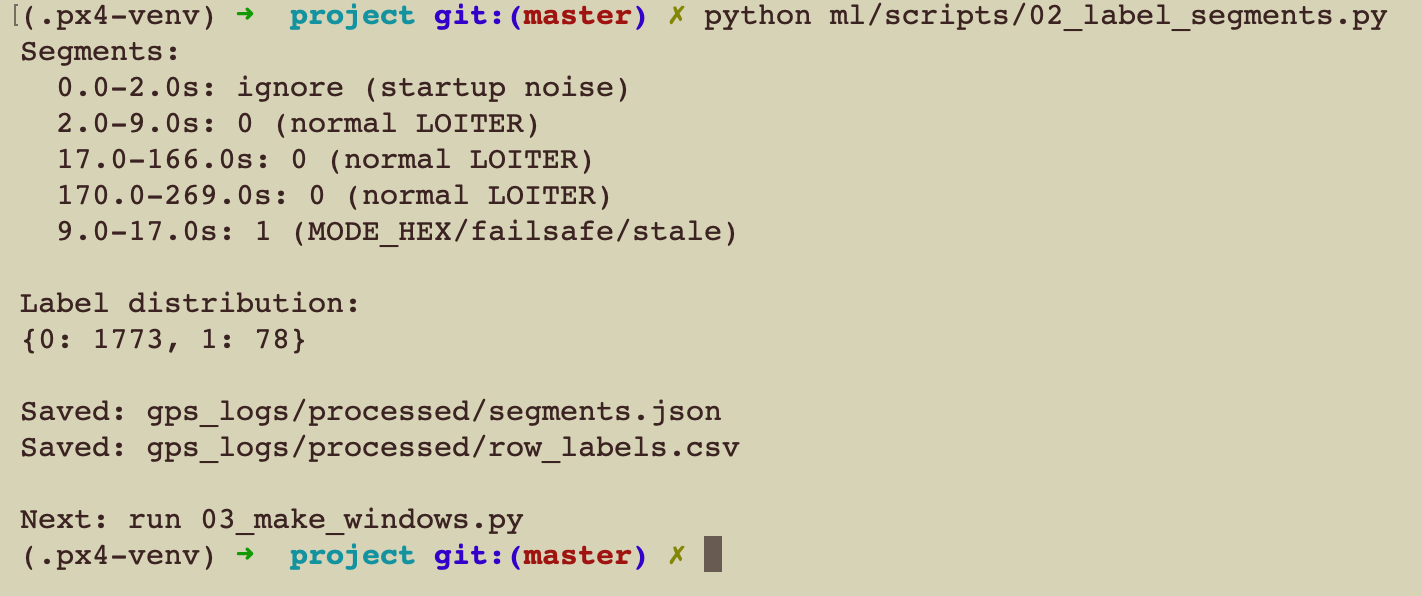
\includegraphics[width=0.7\linewidth]{figures/label segments.png}
    \caption{Label segment annotations applied to telemetry data}
    \label{fig:label_segments}
\end{figure}

\begin{figure}[htbp]
    \centering
    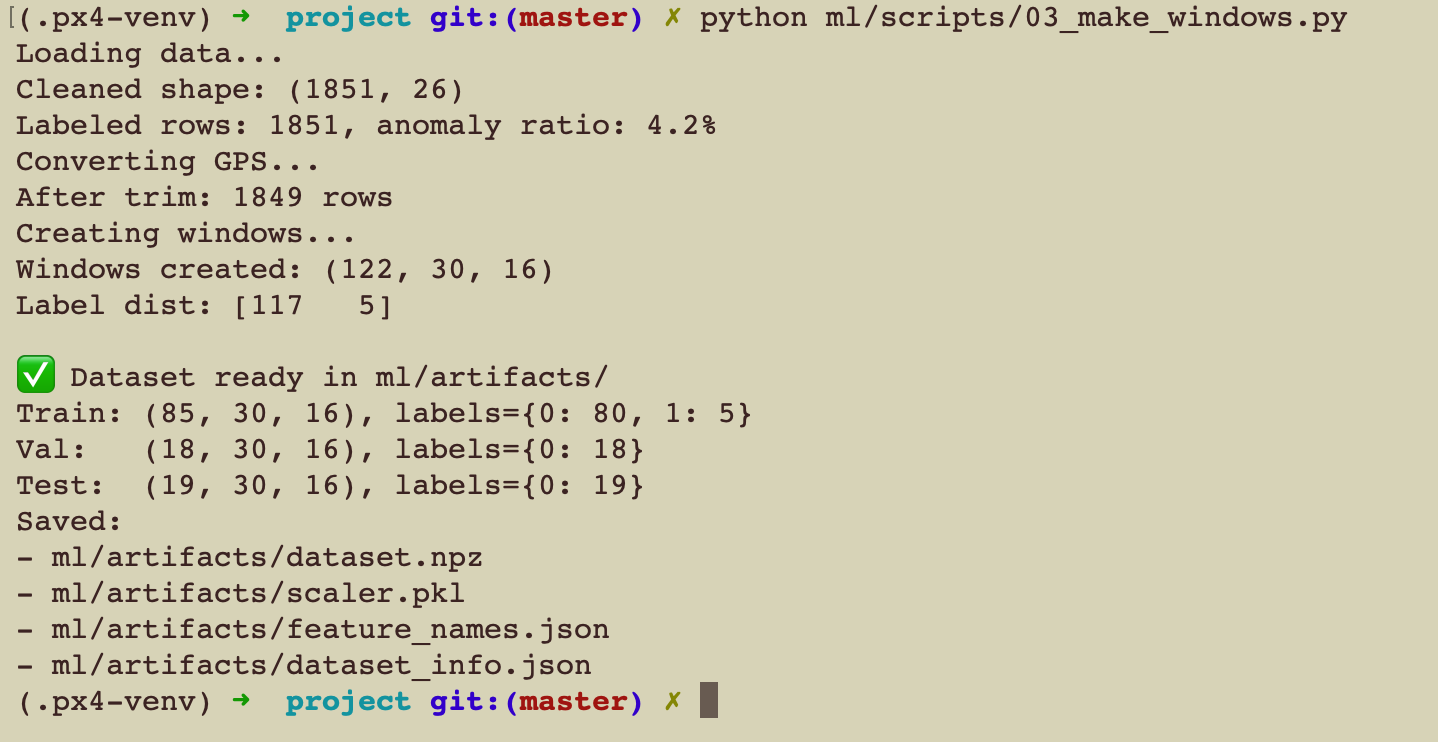
\includegraphics[width=0.7\linewidth]{figures/make the windows for train valuation and testing.png}
    \caption{Sliding window generation pipeline for train/val/test splits}
    \label{fig:windows}
\end{figure}

\subsection{5.3.4 Live Inference Engine}

Real-time detection using trained models:

\begin{lstlisting}[language=python, style=pythonstyle]
# Step_4_Detection/ml/live_inference.py
from collections import deque
import numpy as np

class LiveAnomalyDetector:
    def __init__(self, model_path, scaler_path):
        self.model = joblib.load(model_path)
        self.scaler = joblib.load(scaler_path)
        self.buffer = deque(maxlen=30)  # 3-second window @ 10Hz
        
    def extract_features(self, msg_dict):
        features = [
            msg['x_m'], msg['y_m'], msg['alt_m'], msg['rel_alt_m'],
            msg['vel_m_s'], msg['hdg_deg'], msg['fix_type'],
            msg['satellites_visible'], msg['eph_m'], msg['epv_m'],
            # ... 34 total features
        ]
        return features
        
    def predict(self):
        if len(self.buffer) >= 30:
            window = np.stack(self.buffer)
            window_scaled = self.scaler.transform(window.reshape(1, -1))
            probability = self.model.predict_proba(window_scaled)[0, 1]
            return probability
        return None
\end{lstlisting}

\textbf{Inference Pipeline}:
\begin{itemize}
    \item 30-message sliding buffer (3 seconds @ 10Hz)
    \item Feature extraction from MAVLink stream
    \item Stacked window creation
    \item Model prediction with probability output
\item Real-time logging to CSV
\end{itemize}

\begin{figure}[htbp]
    \centering
    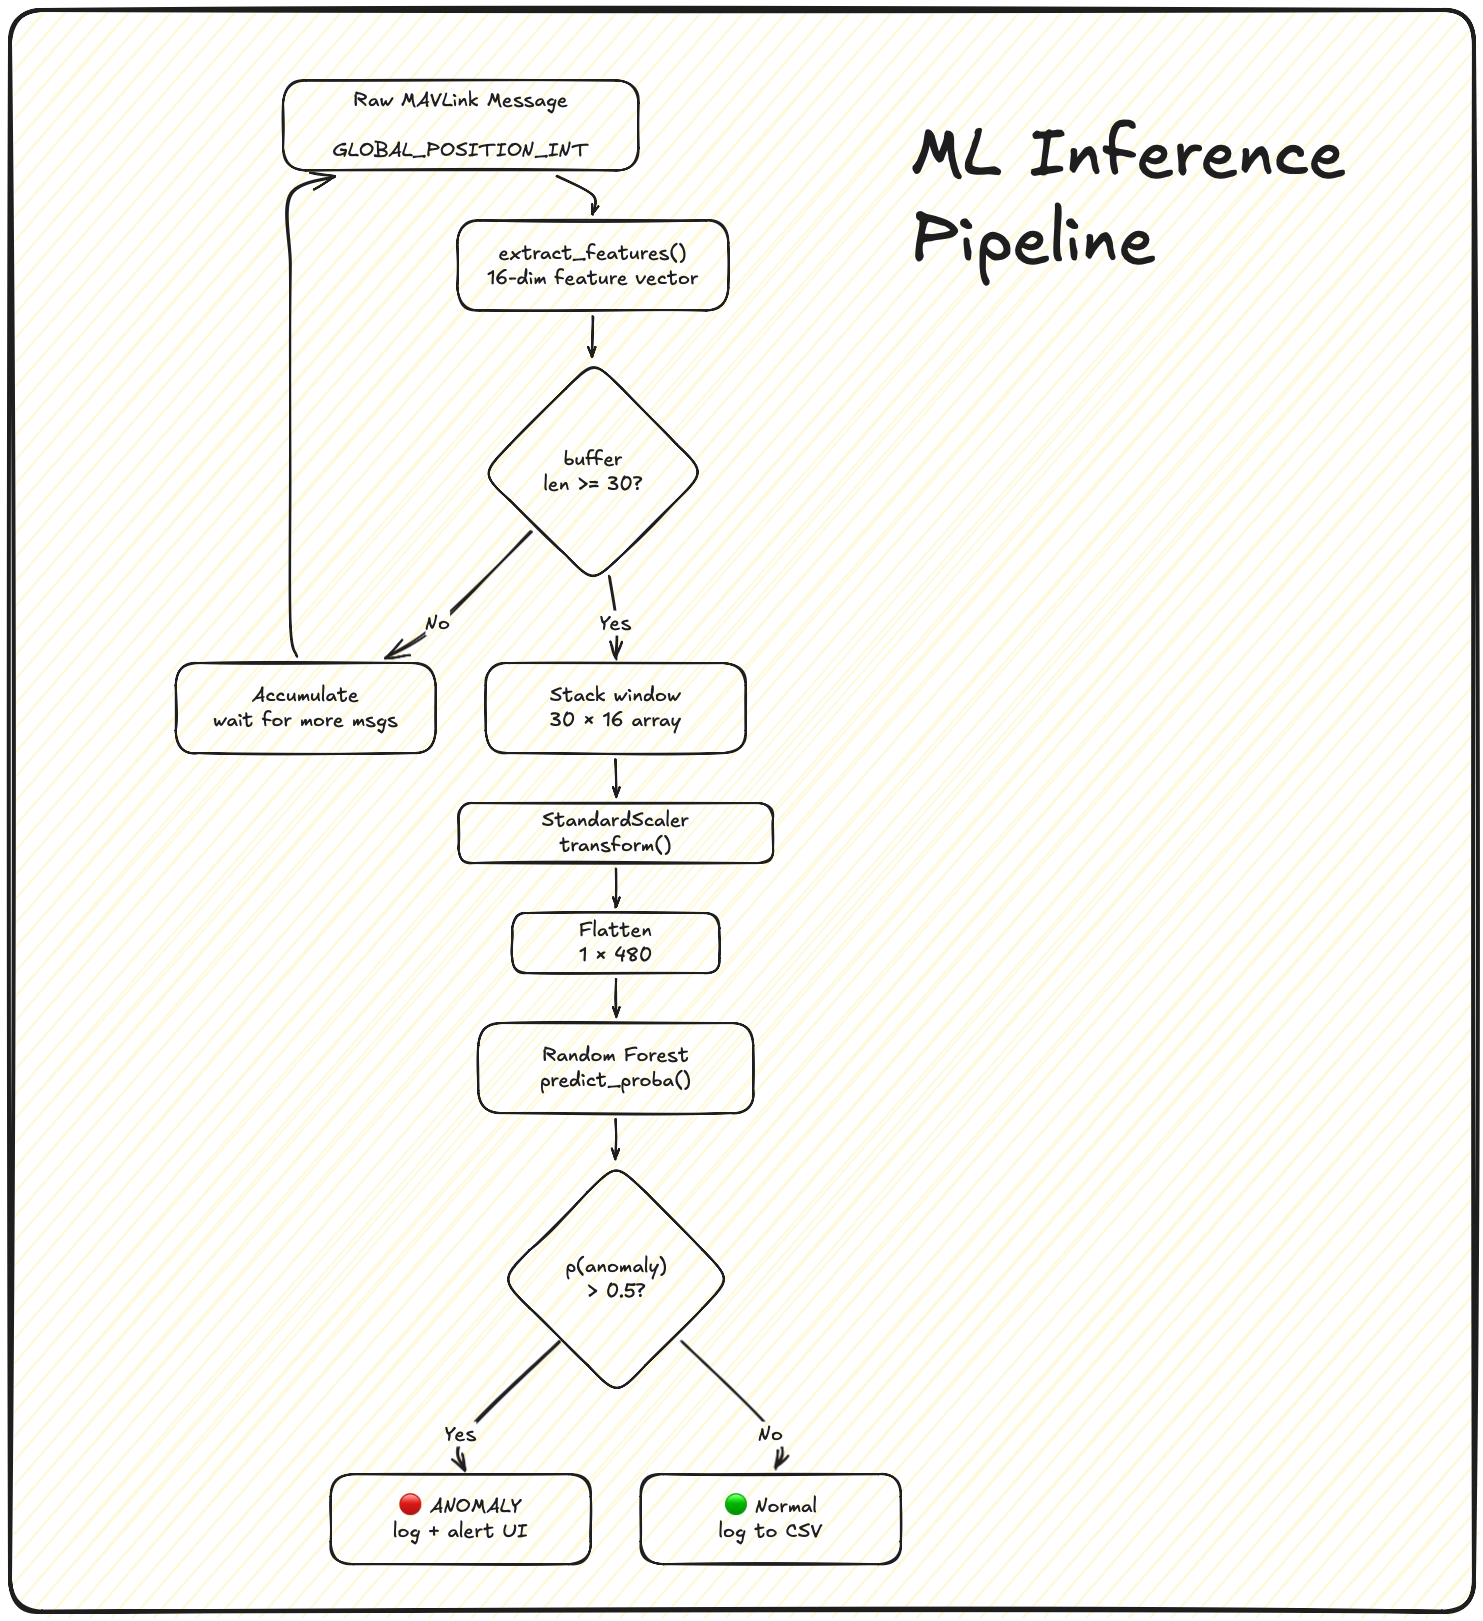
\includegraphics[width=0.7\linewidth]{figures/ML Inference Pipeline Diagram.png}
    \caption{ML inference pipeline diagram}
    \label{fig:inference_pipeline}
\end{figure}

\subsection{5.3.5 Streamlit Dashboard}

Web-based monitoring interface:

\textbf{Dashboard Features}:
\begin{itemize}
    \item Live GPS Trust Index (0-1 scale)
    \item Real-time telemetry display
    \item Historical log replay
    \item Anomaly alerts
    \item Detection confidence metrics
    \item Auto-refresh from live log files
\end{itemize}

\begin{figure}[htbp]
    \centering
    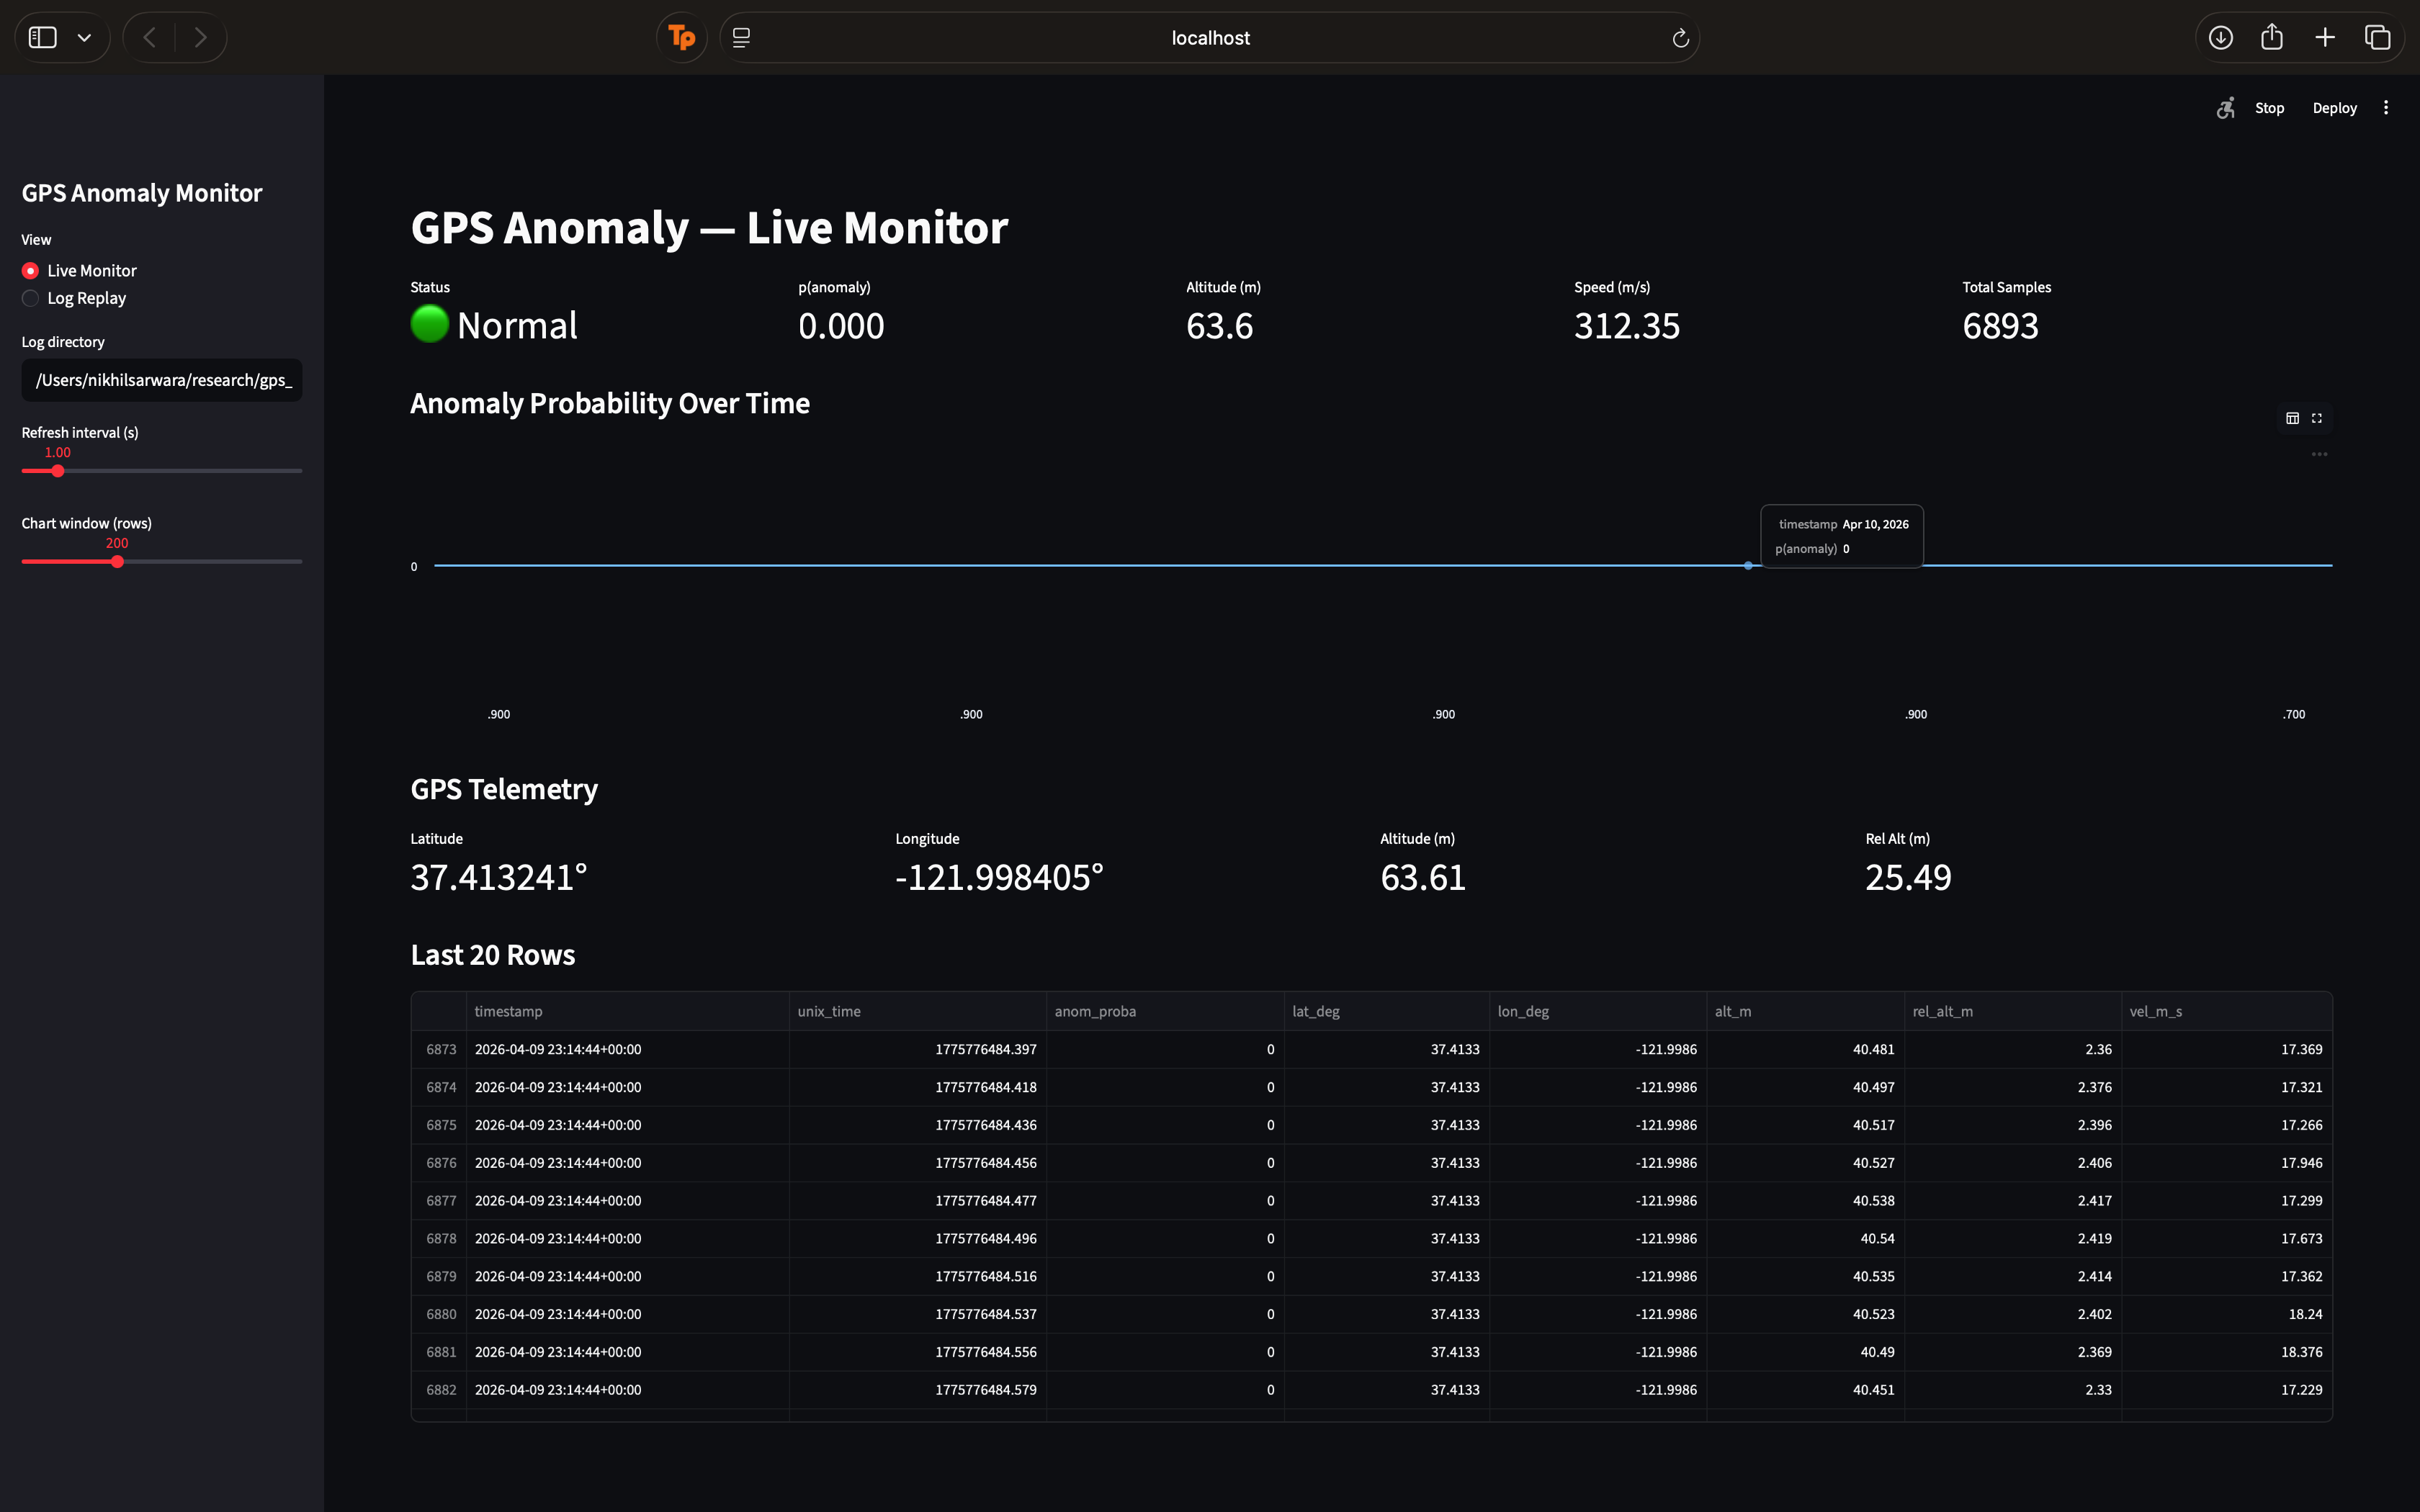
\includegraphics[width=0.7\linewidth]{figures/streamlit ui running live detection.png}
    \caption{Streamlit live detection dashboard}
    \label{fig:streamlit}
\end{figure}

\begin{figure}[htbp]
    \centering
    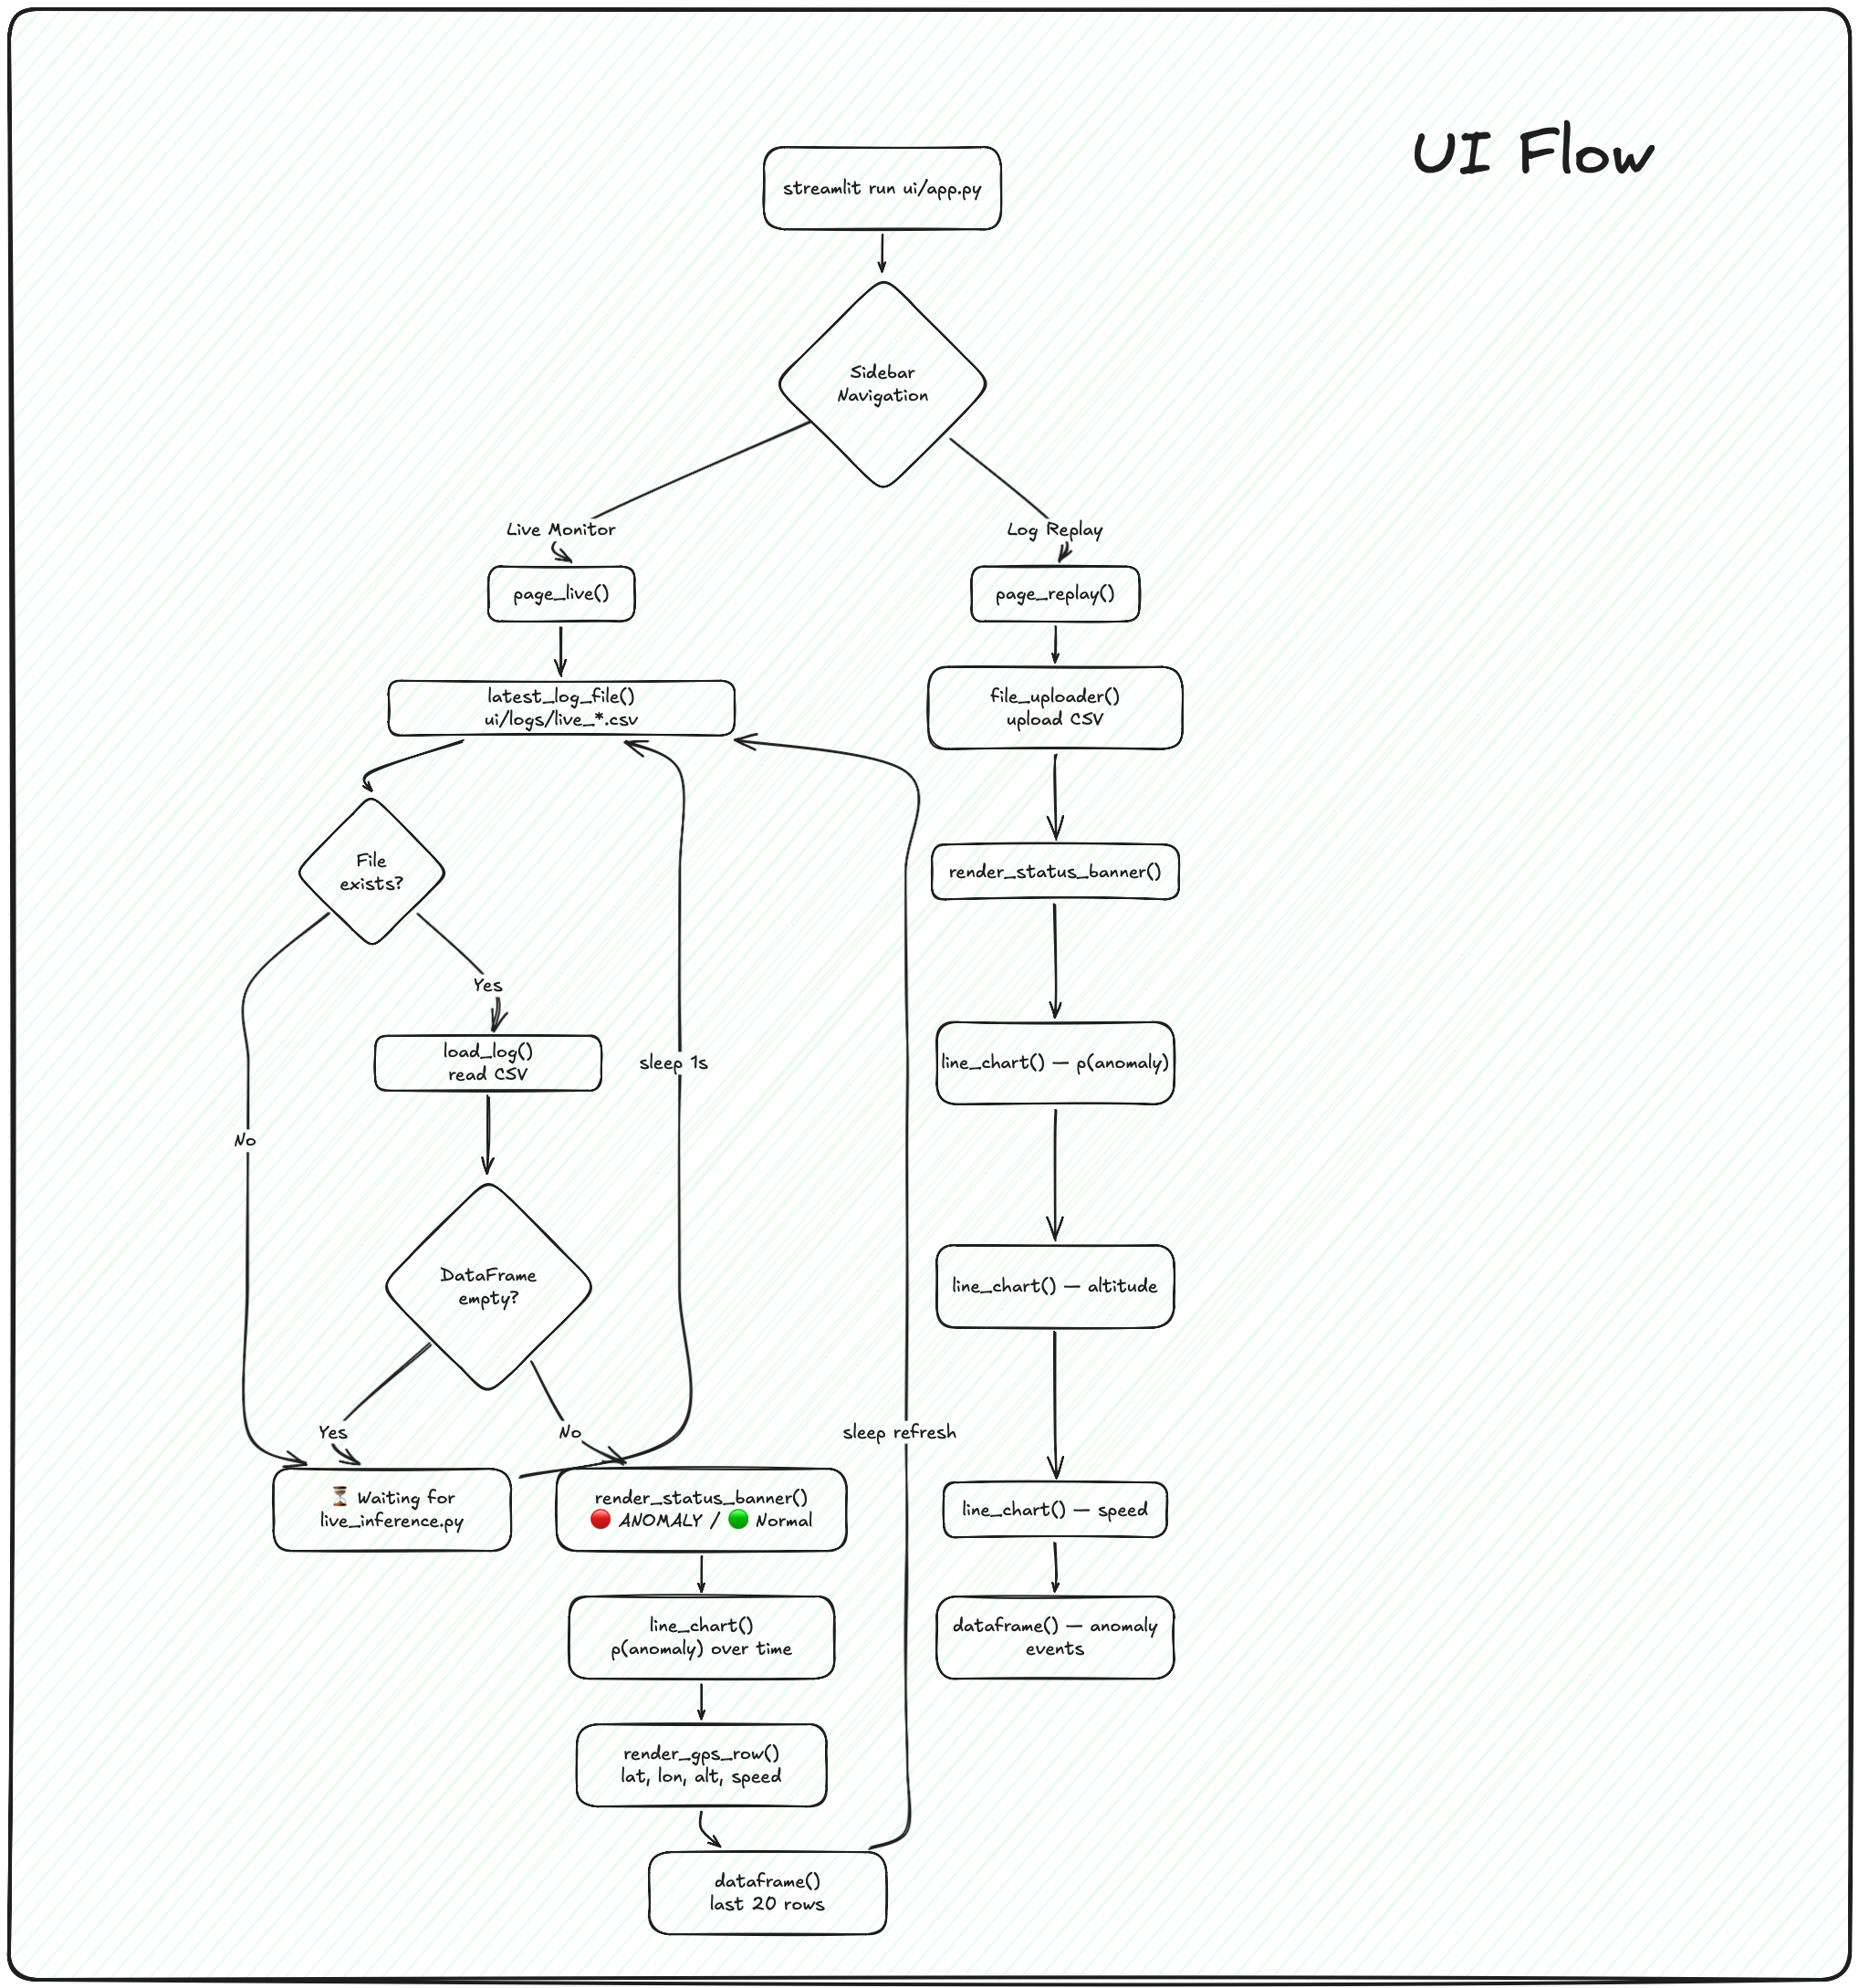
\includegraphics[width=0.7\linewidth]{figures/UI Flow Diagram.png}
    \caption{Streamlit UI flow diagram}
    \label{fig:ui_flow}
\end{figure}

\subsection{5.3.6 TUI Management Interface}

Terminal-based system management:

\textbf{TUI Features}:
\begin{itemize}
    \item Interactive component selector with status dashboard
    \item GPS Monitor, Live Inference, Dashboard, PX4 simulation controls
    \item Start/Stop individual components
    \item Start All / Stop All batch operations
    \item ML Pipeline buttons (Process, Train, Full)
    \item Kill Gazebo for simulation cleanup
    \item Data file information display
    \item View live logs for any component
    \item PID management and process lifecycle
\end{itemize}

\begin{figure}[htbp]
    \centering
    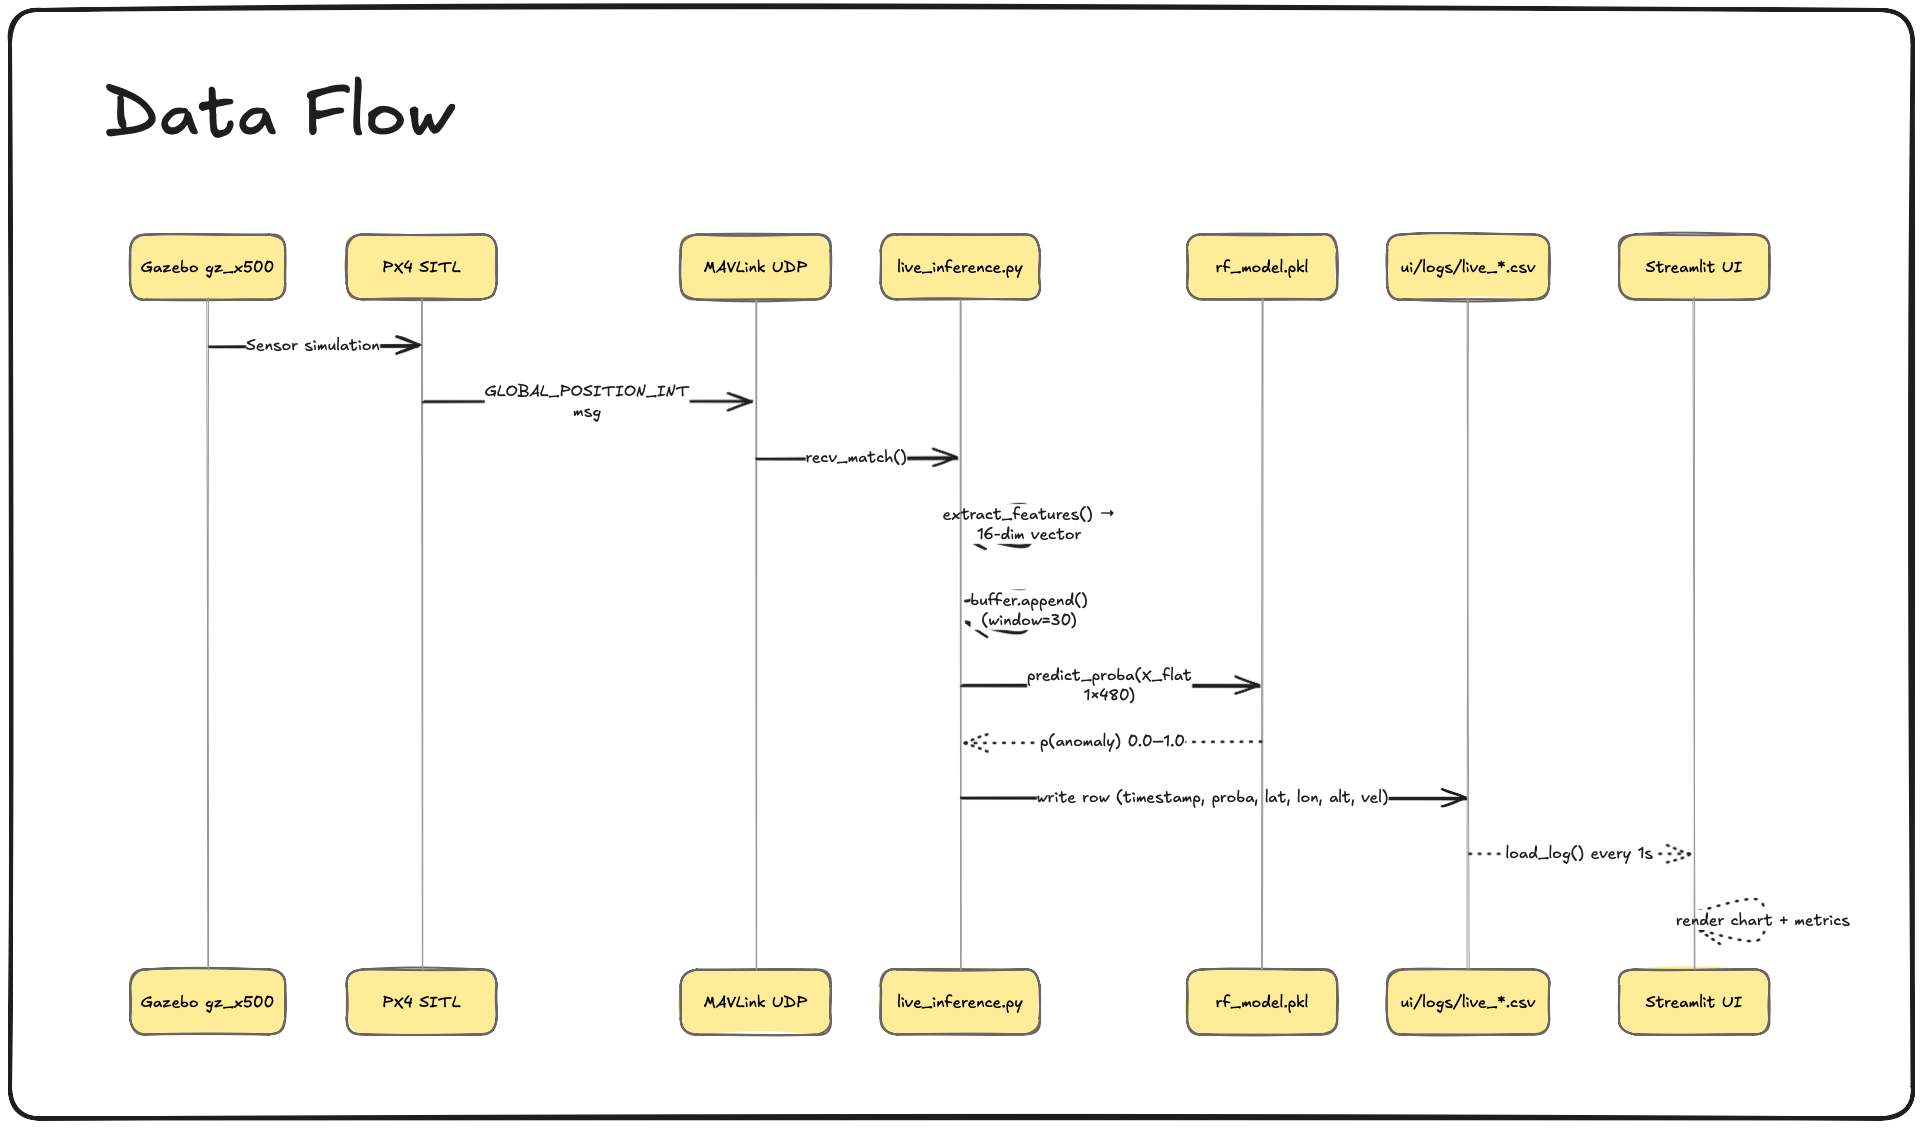
\includegraphics[width=0.7\linewidth]{figures/Data Flow Diagram.png}
    \caption{System data flow diagram}
    \label{fig:data_flow}
\end{figure}

